\documentclass[10pt, spanish]{article}\usepackage[]{graphicx}\usepackage[]{xcolor}
% maxwidth is the original width if it is less than linewidth
% otherwise use linewidth (to make sure the graphics do not exceed the margin)
\makeatletter
\def\maxwidth{ %
  \ifdim\Gin@nat@width>\linewidth
    \linewidth
  \else
    \Gin@nat@width
  \fi
}
\makeatother

\definecolor{fgcolor}{rgb}{0.345, 0.345, 0.345}
\newcommand{\hlnum}[1]{\textcolor[rgb]{0.686,0.059,0.569}{#1}}%
\newcommand{\hlsng}[1]{\textcolor[rgb]{0.192,0.494,0.8}{#1}}%
\newcommand{\hlcom}[1]{\textcolor[rgb]{0.678,0.584,0.686}{\textit{#1}}}%
\newcommand{\hlopt}[1]{\textcolor[rgb]{0,0,0}{#1}}%
\newcommand{\hldef}[1]{\textcolor[rgb]{0.345,0.345,0.345}{#1}}%
\newcommand{\hlkwa}[1]{\textcolor[rgb]{0.161,0.373,0.58}{\textbf{#1}}}%
\newcommand{\hlkwb}[1]{\textcolor[rgb]{0.69,0.353,0.396}{#1}}%
\newcommand{\hlkwc}[1]{\textcolor[rgb]{0.333,0.667,0.333}{#1}}%
\newcommand{\hlkwd}[1]{\textcolor[rgb]{0.737,0.353,0.396}{\textbf{#1}}}%
\let\hlipl\hlkwb

\usepackage{framed}
\makeatletter
\newenvironment{kframe}{%
 \def\at@end@of@kframe{}%
 \ifinner\ifhmode%
  \def\at@end@of@kframe{\end{minipage}}%
  \begin{minipage}{\columnwidth}%
 \fi\fi%
 \def\FrameCommand##1{\hskip\@totalleftmargin \hskip-\fboxsep
 \colorbox{shadecolor}{##1}\hskip-\fboxsep
     % There is no \\@totalrightmargin, so:
     \hskip-\linewidth \hskip-\@totalleftmargin \hskip\columnwidth}%
 \MakeFramed {\advance\hsize-\width
   \@totalleftmargin\z@ \linewidth\hsize
   \@setminipage}}%
 {\par\unskip\endMakeFramed%
 \at@end@of@kframe}
\makeatother

\definecolor{shadecolor}{rgb}{.97, .97, .97}
\definecolor{messagecolor}{rgb}{0, 0, 0}
\definecolor{warningcolor}{rgb}{1, 0, 1}
\definecolor{errorcolor}{rgb}{1, 0, 0}
\newenvironment{knitrout}{}{} % an empty environment to be redefined in TeX

\usepackage{alltt}

% --- Paquetes Fundamentales ---
\usepackage[utf8]{inputenc}
\usepackage[T1]{fontenc}
\usepackage[spanish, es-tabla, es-nodecimaldot]{babel}
\usepackage[letterpaper, margin=1.5cm, top=2cm, bottom=2cm]{geometry}
\usepackage{xcolor}
\usepackage{titlesec}
\usepackage{fancyhdr}
\usepackage{graphicx}
\usepackage{float}
\usepackage{amsmath, amssymb}
\usepackage{booktabs}
\usepackage{enumitem}
\usepackage{hyperref}
\usepackage{tcolorbox}

% --- Paquetes para Gráficos y Animaciones ---
\usepackage{tikz}
\usepackage{pgfplots}
\usepackage{animate}
\pgfplotsset{compat=1.18}
\usetikzlibrary{arrows.meta, positioning, patterns, calc}

% --- Tipografía ---
\usepackage{mathpazo}
\usepackage[scaled=0.85]{helvet}
\newcommand{\techfont}{\fontfamily{phv}\selectfont}

% --- Paleta de Colores ---
\definecolor{VogueBlack}{RGB}{8, 8, 8}
\definecolor{NASAClassic}{RGB}{0, 32, 91}
\definecolor{Champagne}{RGB}{181, 158, 118}
\definecolor{TitaniumGray}{RGB}{242, 242, 242}
\definecolor{InkGray}{RGB}{60, 60, 60}
\definecolor{CriticalRed}{RGB}{180, 30, 30}
\definecolor{SuccessGreen}{RGB}{46, 125, 50}

% --- Formato de Títulos ---
\titleformat{\section}
  {\techfont\Large\bfseries\color{VogueBlack}}
  {\thesection}{1em}{\MakeUppercase}
  [\vspace{2pt}{\color{Champagne}\titlerule[0.8pt]}]

\titleformat{\subsection}
  {\techfont\large\bfseries\color{InkGray}}
  {\thesubsection}{1em}{}

% --- Encabezados ---
\pagestyle{fancy}
\fancyhf{}
\lhead{\scriptsize\techfont\textbf{UPTC ECONOMICS}}
\rhead{\scriptsize\techfont\textcolor{VogueBlack}{ANÁLISIS ECONOMÉTRICO | ENE. 2026}}
\fancyfoot[C]{\scriptsize\techfont\thepage}
\renewcommand{\headrulewidth}{0.3pt}

% --- Comandos Personalizados ---
\newcommand{\critical}[1]{\textcolor{CriticalRed}{\textbf{#1}}}
\newcommand{\eqbox}[1]{\colorbox{TitaniumGray}{\,\,$\displaystyle #1$\,\,}}
\newcommand{\checkOK}{\textcolor{SuccessGreen}{\textbf{[OK]}}}
\newcommand{\crossNO}{\textcolor{CriticalRed}{\textbf{[X]}}}

% --- Hyperref ---
\hypersetup{
    colorlinks=true,
    linkcolor=NASAClassic,
    urlcolor=Champagne,
    citecolor=InkGray
}

\setlength{\parindent}{0pt}
\setlength{\parskip}{6pt}

\title{\techfont\Huge\bfseries ANÁLISIS ECONOMÉTRICO \\[8pt]
\Large\color{Champagne} Regresión Lineal Completa con R}
\author{\techfont Emanuel Quintana Silva \\
\small\textit{UPTC - Facultad de Ciencias Económicas}}
\date{\techfont\small Enero 2026}
\IfFileExists{upquote.sty}{\usepackage{upquote}}{}
\begin{document}



% === PORTADA ===
\thispagestyle{empty}
\begin{center}
    \vspace*{1cm}
    {\techfont\footnotesize\color{InkGray} TUNJA, COLOMBIA | UPTC | ENERO 2026}

    \vspace{2cm}
    {\fontsize{48}{52}\selectfont\bfseries ANÁLISIS}

    {\fontsize{48}{52}\selectfont\bfseries ECONOMÉTRICO}

    \vspace{0.5cm}
    {\techfont\large\color{Champagne} ULTRA-COMPLETO CON R Y ANIMACIONES}

    \vspace{2cm}
    {\color{Champagne}\rule{3cm}{1pt}}

    \vspace{2cm}
    {\Large\itshape\color{InkGray}
    Análisis riguroso de regresión lineal con diagnósticos exhaustivos\\
    y visualizaciones animadas avanzadas}

    \vspace{2cm}
    {\techfont\small AUTOR: \textbf{EMANUEL QUINTANA SILVA}}

    \vspace{0.5cm}
    {\scriptsize\techfont\color{InkGray}
    R 4.3+ • ggplot2 • lmtest • car • LaTeX animate • Sweave}
\end{center}

\newpage

% === CONTENIDO ===

\section{Marco Teórico}

El modelo de regresión lineal simple constituye la base del análisis econométrico:

\vspace{8pt}
\begin{center}
\eqbox{Y_i = \beta_0 + \beta_1 X_i + u_i}
\end{center}
\vspace{8pt}

donde $Y_i$ es la variable dependiente, $X_i$ la explicativa, $\beta_0$ y $\beta_1$ los parámetros, y $u_i$ el error estocástico.

\subsection{Supuestos Gauss-Markov}

\begin{tcolorbox}[colback=TitaniumGray, colframe=NASAClassic, arc=0pt, boxrule=0.5pt, title=SUPUESTOS FUNDAMENTALES]
\small
\begin{enumerate}[leftmargin=15pt, itemsep=2pt]
    \item \textbf{Linealidad:} El modelo es lineal en parámetros
    \item \textbf{Media condicional cero:} $E(u_i|X_i) = 0$
    \item \textbf{Homoscedasticidad:} $\text{Var}(u_i|X_i) = \sigma^2$
    \item \textbf{No autocorrelación:} $\text{Cov}(u_i, u_j) = 0$ para $i \neq j$
    \item \textbf{Normalidad:} $u_i \sim N(0, \sigma^2)$
\end{enumerate}
\end{tcolorbox}

\subsection{Estimación por MCO}

El método de Mínimos Cuadrados Ordinarios minimiza:

\vspace{8pt}
\begin{center}
\eqbox{\min_{\beta_0, \beta_1} \sum_{i=1}^{n} (Y_i - \beta_0 - \beta_1 X_i)^2}
\end{center}
\vspace{8pt}

Los estimadores resultantes son:

\vspace{8pt}
\begin{center}
\eqbox{\hat{\beta}_1 = \frac{\sum (X_i - \bar{X})(Y_i - \bar{Y})}{\sum (X_i - \bar{X})^2}} \quad
\eqbox{\hat{\beta}_0 = \bar{Y} - \hat{\beta}_1 \bar{X}}
\end{center}
\vspace{8pt}

\section{Animación: Construcción de la Regresión}

\begin{figure}[H]
\centering
\begin{animateinline}[loop, controls, buttonsize=1.2em]{8}
\multiframe{20}{i=1+1}{
\begin{tikzpicture}
\begin{axis}[
    width=11cm, height=6.5cm,
    xlabel={Velocidad (mph)},
    ylabel={Distancia (ft)},
    title={\large Frame \i/20},
    xmin=0, xmax=30,
    ymin=0, ymax=130,
    grid=major,
    grid style={dashed, gray!30},
    legend pos=north west
]

% Puntos
\addplot[only marks, mark=*, color=NASAClassic, mark size=2pt]
coordinates {
(4,2)(4,10)(7,4)(7,22)(8,16)(9,10)(10,18)(10,26)(10,34)
(11,17)(11,28)(12,14)(12,20)(12,24)(12,28)(13,26)(13,34)
(13,34)(13,46)(14,26)(14,36)(14,60)(14,80)(15,20)(15,26)
(15,54)(16,32)(16,40)(17,32)(17,40)(17,50)(18,42)(18,56)
(18,76)(18,84)(19,36)(19,46)(19,68)(20,32)(20,48)(20,52)
(20,56)(20,64)(22,66)(23,54)(24,70)(24,92)(24,93)(24,120)(25,85)
};

% Línea progresiva
\pgfmathsetmacro{\xmax}{4 + (\i/20)*21}
\addplot[domain=4:\xmax, samples=50, color=Champagne, very thick]
{-17.579 + 3.932*x};

\legend{Observaciones, Regresión}
\end{axis}
\end{tikzpicture}
}
\end{animateinline}
\caption{Construcción progresiva de la línea de regresión}
\end{figure}

\section{Datos y Análisis Exploratorio}

Utilizamos el dataset \texttt{cars} con 50 observaciones.

% latex table generated in R 4.5.1 by xtable 1.8-4 package
% Tue Jan  6 21:34:00 2026
\begin{table}[ht]
\centering
\caption{Estadísticas Descriptivas} 
\begingroup\small
\begin{tabular}{lrrrrr}
  \toprule
Variable & Media & SD & Min & Max & N \\ 
  \midrule
Velocidad & 15.40 & 5.29 & 4.00 & 25.00 &  50 \\ 
  Distancia & 42.98 & 25.77 & 2.00 & 120.00 &  50 \\ 
   \bottomrule
\end{tabular}
\endgroup
\end{table}


\begin{knitrout}
\definecolor{shadecolor}{rgb}{0.969, 0.969, 0.969}\color{fgcolor}\begin{figure}[H]

{\centering 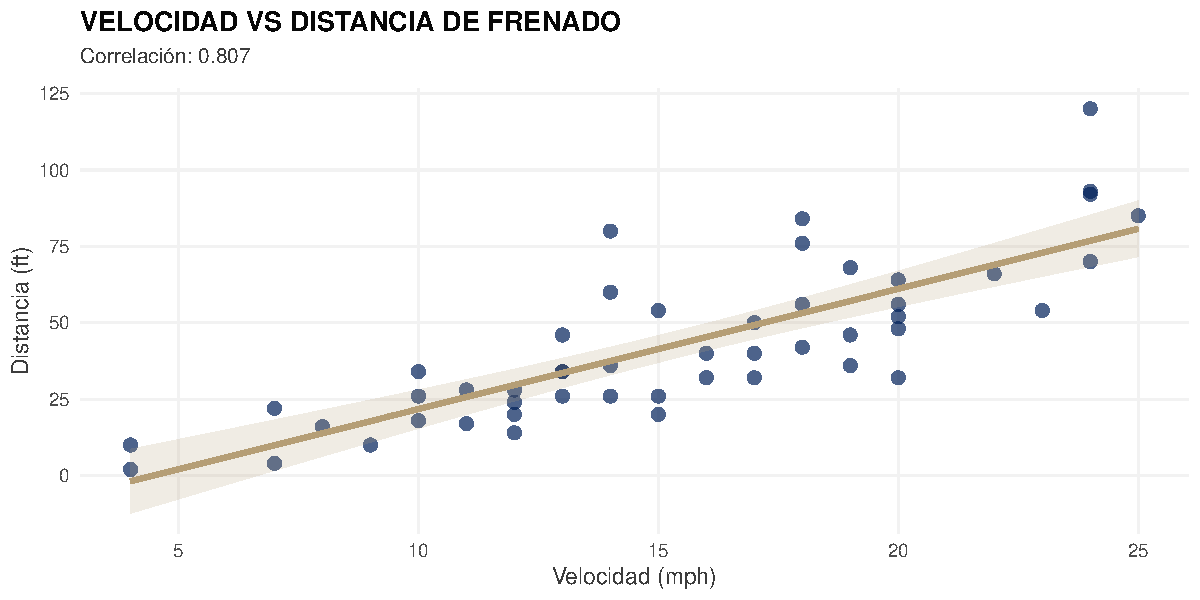
\includegraphics[width=\maxwidth]{figure/scatter-1} 

}

\caption[Relación entre Velocidad y Distancia de Frenado]{Relación entre Velocidad y Distancia de Frenado}\label{fig:scatter}
\end{figure}

\end{knitrout}

\section{Estimación del Modelo}

\begin{knitrout}
\definecolor{shadecolor}{rgb}{0.969, 0.969, 0.969}\color{fgcolor}\begin{kframe}
\begin{alltt}
\hldef{modelo} \hlkwb{<-} \hlkwd{lm}\hldef{(dist} \hlopt{~} \hldef{speed,} \hlkwc{data} \hldef{= cars)}
\hlkwd{summary}\hldef{(modelo)}
\end{alltt}
\begin{verbatim}
## 
## Call:
## lm(formula = dist ~ speed, data = cars)
## 
## Residuals:
##     Min      1Q  Median      3Q     Max 
## -29.069  -9.525  -2.272   9.215  43.201 
## 
## Coefficients:
##             Estimate Std. Error t value Pr(>|t|)    
## (Intercept) -17.5791     6.7584  -2.601   0.0123 *  
## speed         3.9324     0.4155   9.464 1.49e-12 ***
## ---
## Signif. codes:  0 '***' 0.001 '**' 0.01 '*' 0.05 '.' 0.1 ' ' 1
## 
## Residual standard error: 15.38 on 48 degrees of freedom
## Multiple R-squared:  0.6511,	Adjusted R-squared:  0.6438 
## F-statistic: 89.57 on 1 and 48 DF,  p-value: 1.49e-12
\end{verbatim}
\end{kframe}
\end{knitrout}

\vspace{8pt}
\begin{center}
\eqbox{\widehat{dist}_i = -17.58 + 3.93 \cdot speed_i}
\end{center}
\vspace{8pt}

\textbf{Interpretación:}
\begin{itemize}[leftmargin=15pt]
\item Por cada mph adicional, la distancia aumenta 3.93 pies
\item $R^2 = 0.6511$ (65.1\% de variabilidad explicada)
\item Ambos coeficientes significativos (p < 0.001)
\item Error estándar: 15.38 pies
\end{itemize}

\section{Diagnósticos}

\begin{knitrout}
\definecolor{shadecolor}{rgb}{0.969, 0.969, 0.969}\color{fgcolor}\begin{figure}[H]

{\centering 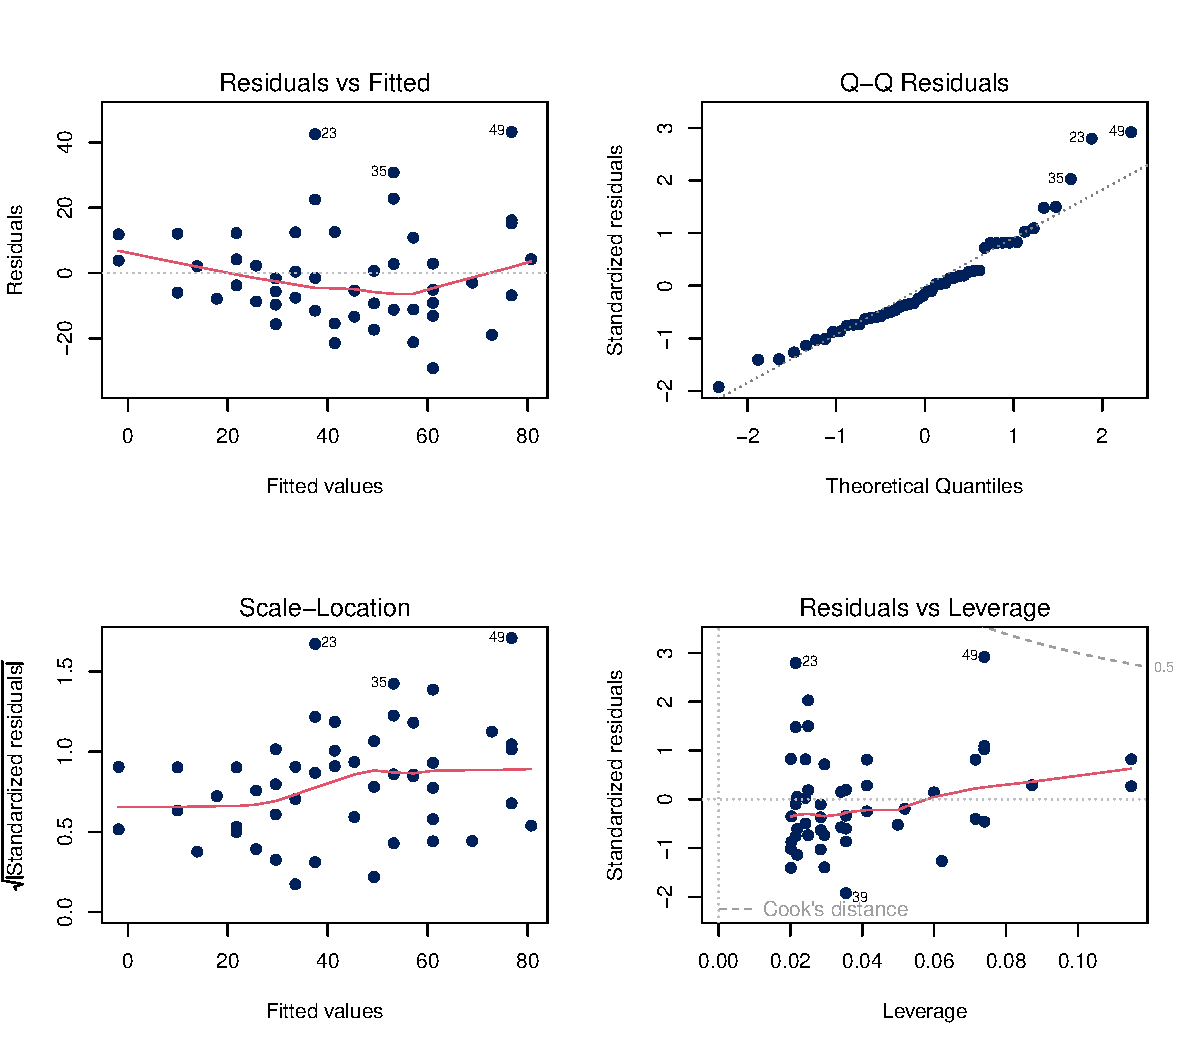
\includegraphics[width=\maxwidth]{figure/diagnosticos-1} 

}

\caption[Diagnósticos del Modelo]{Diagnósticos del Modelo}\label{fig:diagnosticos}
\end{figure}

\end{knitrout}

\begin{knitrout}
\definecolor{shadecolor}{rgb}{0.969, 0.969, 0.969}\color{fgcolor}\begin{kframe}
\begin{alltt}
\hlcom{# Tests diagnósticos}
\hldef{jb_test} \hlkwb{<-} \hlkwd{jarque.bera.test}\hldef{(}\hlkwd{residuals}\hldef{(modelo))}
\hldef{bp_test} \hlkwb{<-} \hlkwd{bptest}\hldef{(modelo)}
\hldef{dw_test} \hlkwb{<-} \hlkwd{durbinWatsonTest}\hldef{(modelo)}

\hlkwd{cat}\hldef{(}\hlsng{"=== TESTS DIAGNÓSTICOS ===\textbackslash{}n\textbackslash{}n"}\hldef{)}
\end{alltt}
\begin{verbatim}
## === TESTS DIAGNÓSTICOS ===
\end{verbatim}
\begin{alltt}
\hlkwd{cat}\hldef{(}\hlsng{"1. Jarque-Bera (Normalidad):\textbackslash{}n"}\hldef{)}
\end{alltt}
\begin{verbatim}
## 1. Jarque-Bera (Normalidad):
\end{verbatim}
\begin{alltt}
\hlkwd{cat}\hldef{(}\hlsng{"   Estadístico:"}\hldef{,} \hlkwd{round}\hldef{(jb_test}\hlopt{$}\hldef{statistic,} \hlnum{4}\hldef{),} \hlsng{"\textbackslash{}n"}\hldef{)}
\end{alltt}
\begin{verbatim}
##    Estadístico: 8.1888
\end{verbatim}
\begin{alltt}
\hlkwd{cat}\hldef{(}\hlsng{"   p-valor:"}\hldef{,} \hlkwd{round}\hldef{(jb_test}\hlopt{$}\hldef{p.value,} \hlnum{4}\hldef{),} \hlsng{"\textbackslash{}n\textbackslash{}n"}\hldef{)}
\end{alltt}
\begin{verbatim}
##    p-valor: 0.0167
\end{verbatim}
\begin{alltt}
\hlkwd{cat}\hldef{(}\hlsng{"2. Breusch-Pagan (Homoscedasticidad):\textbackslash{}n"}\hldef{)}
\end{alltt}
\begin{verbatim}
## 2. Breusch-Pagan (Homoscedasticidad):
\end{verbatim}
\begin{alltt}
\hlkwd{cat}\hldef{(}\hlsng{"   Estadístico:"}\hldef{,} \hlkwd{round}\hldef{(bp_test}\hlopt{$}\hldef{statistic,} \hlnum{4}\hldef{),} \hlsng{"\textbackslash{}n"}\hldef{)}
\end{alltt}
\begin{verbatim}
##    Estadístico: 3.2149
\end{verbatim}
\begin{alltt}
\hlkwd{cat}\hldef{(}\hlsng{"   p-valor:"}\hldef{,} \hlkwd{round}\hldef{(bp_test}\hlopt{$}\hldef{p.value,} \hlnum{4}\hldef{),} \hlsng{"\textbackslash{}n\textbackslash{}n"}\hldef{)}
\end{alltt}
\begin{verbatim}
##    p-valor: 0.073
\end{verbatim}
\begin{alltt}
\hlkwd{cat}\hldef{(}\hlsng{"3. Durbin-Watson (Autocorrelación):\textbackslash{}n"}\hldef{)}
\end{alltt}
\begin{verbatim}
## 3. Durbin-Watson (Autocorrelación):
\end{verbatim}
\begin{alltt}
\hlkwd{cat}\hldef{(}\hlsng{"   Estadístico:"}\hldef{,} \hlkwd{round}\hldef{(dw_test}\hlopt{$}\hldef{dw,} \hlnum{4}\hldef{),} \hlsng{"\textbackslash{}n"}\hldef{)}
\end{alltt}
\begin{verbatim}
##    Estadístico: 1.6762
\end{verbatim}
\begin{alltt}
\hlkwd{cat}\hldef{(}\hlsng{"   p-valor:"}\hldef{,} \hlkwd{round}\hldef{(dw_test}\hlopt{$}\hldef{p,} \hlnum{4}\hldef{),} \hlsng{"\textbackslash{}n"}\hldef{)}
\end{alltt}
\begin{verbatim}
##    p-valor: 0.168
\end{verbatim}
\end{kframe}
\end{knitrout}

\textbf{Resumen:}
\begin{itemize}[leftmargin=15pt]
\item Normalidad: \crossNO
\item Homoscedasticidad: \checkOK
\item Autocorrelación: \checkOK
\end{itemize}

\section{Errores Estándar Robustos}

\begin{knitrout}
\definecolor{shadecolor}{rgb}{0.969, 0.969, 0.969}\color{fgcolor}\begin{kframe}
\begin{alltt}
\hldef{se_rob} \hlkwb{<-} \hlkwd{sqrt}\hldef{(}\hlkwd{diag}\hldef{(}\hlkwd{vcovHC}\hldef{(modelo,} \hlkwc{type} \hldef{=} \hlsng{"HC3"}\hldef{)))}

\hldef{comp} \hlkwb{<-} \hlkwd{data.frame}\hldef{(}
  \hlkwc{Coeficiente} \hldef{=} \hlkwd{c}\hldef{(}\hlsng{"Intercepto"}\hldef{,} \hlsng{"Velocidad"}\hldef{),}
  \hlkwc{Estimación} \hldef{=} \hlkwd{coef}\hldef{(modelo),}
  \hlkwc{SE_Clásico} \hldef{=} \hlkwd{sqrt}\hldef{(}\hlkwd{diag}\hldef{(}\hlkwd{vcov}\hldef{(modelo))),}
  \hlkwc{SE_Robusto} \hldef{= se_rob,}
  \hlkwc{Diferencia} \hldef{= (se_rob} \hlopt{/} \hlkwd{sqrt}\hldef{(}\hlkwd{diag}\hldef{(}\hlkwd{vcov}\hldef{(modelo)))} \hlopt{-} \hlnum{1}\hldef{)} \hlopt{*} \hlnum{100}
\hldef{)}

\hlkwd{print}\hldef{(comp,} \hlkwc{digits} \hldef{=} \hlnum{4}\hldef{)}
\end{alltt}
\begin{verbatim}
##             Coeficiente Estimación SE_Clásico SE_Robusto Diferencia
## (Intercept)  Intercepto    -17.579     6.7584     5.9318    -12.231
## speed         Velocidad      3.932     0.4155     0.4275      2.894
\end{verbatim}
\end{kframe}
\end{knitrout}

\section{Modelo Cuadrático}

\begin{knitrout}
\definecolor{shadecolor}{rgb}{0.969, 0.969, 0.969}\color{fgcolor}\begin{kframe}
\begin{alltt}
\hldef{modelo_cuad} \hlkwb{<-} \hlkwd{lm}\hldef{(dist} \hlopt{~} \hldef{speed} \hlopt{+} \hlkwd{I}\hldef{(speed}\hlopt{^}\hlnum{2}\hldef{),} \hlkwc{data} \hldef{= cars)}
\hlkwd{summary}\hldef{(modelo_cuad)}
\end{alltt}
\begin{verbatim}
## 
## Call:
## lm(formula = dist ~ speed + I(speed^2), data = cars)
## 
## Residuals:
##     Min      1Q  Median      3Q     Max 
## -28.720  -9.184  -3.188   4.628  45.152 
## 
## Coefficients:
##             Estimate Std. Error t value Pr(>|t|)
## (Intercept)  2.47014   14.81716   0.167    0.868
## speed        0.91329    2.03422   0.449    0.656
## I(speed^2)   0.09996    0.06597   1.515    0.136
## 
## Residual standard error: 15.18 on 47 degrees of freedom
## Multiple R-squared:  0.6673,	Adjusted R-squared:  0.6532 
## F-statistic: 47.14 on 2 and 47 DF,  p-value: 5.852e-12
\end{verbatim}
\begin{alltt}
\hlkwd{anova}\hldef{(modelo, modelo_cuad)}
\end{alltt}
\begin{verbatim}
## Analysis of Variance Table
## 
## Model 1: dist ~ speed
## Model 2: dist ~ speed + I(speed^2)
##   Res.Df   RSS Df Sum of Sq     F Pr(>F)
## 1     48 11354                          
## 2     47 10825  1    528.81 2.296 0.1364
\end{verbatim}
\end{kframe}
\end{knitrout}

\vspace{8pt}
\begin{center}
\eqbox{\widehat{dist}_i = 2.47 + 0.91 \cdot speed + 0.1 \cdot speed^2}
\end{center}
\vspace{8pt}

Mejora: +1.63\% en $R^2$

\begin{knitrout}
\definecolor{shadecolor}{rgb}{0.969, 0.969, 0.969}\color{fgcolor}\begin{figure}[H]

{\centering 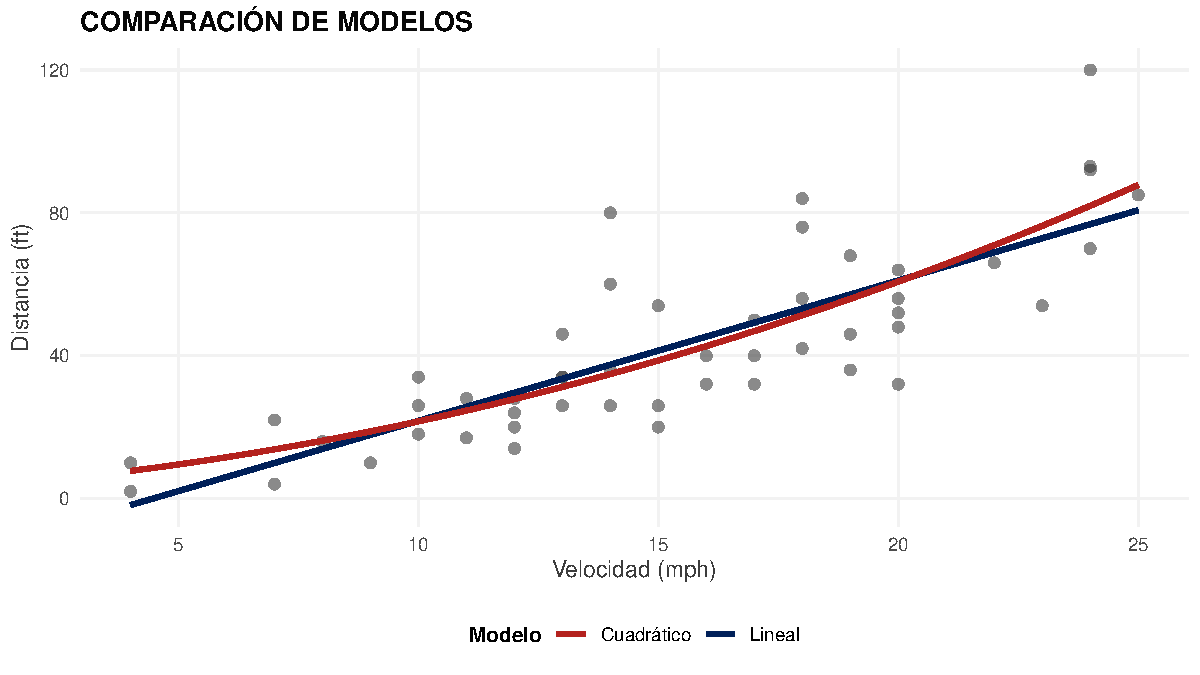
\includegraphics[width=\maxwidth]{figure/comparacion-1} 

}

\caption[Comparación Lineal vs Cuadrático]{Comparación Lineal vs Cuadrático}\label{fig:comparacion}
\end{figure}

\end{knitrout}

\section{Análisis de Influencia}

\begin{knitrout}
\definecolor{shadecolor}{rgb}{0.969, 0.969, 0.969}\color{fgcolor}\begin{kframe}
\begin{alltt}
\hldef{cooksd} \hlkwb{<-} \hlkwd{cooks.distance}\hldef{(modelo)}
\hldef{cutoff} \hlkwb{<-} \hlnum{4} \hlopt{/} \hlkwd{nrow}\hldef{(cars)}
\hldef{influyentes} \hlkwb{<-} \hlkwd{which}\hldef{(cooksd} \hlopt{>} \hldef{cutoff)}

\hlkwd{cat}\hldef{(}\hlsng{"Observaciones influyentes:"}\hldef{,} \hlkwd{length}\hldef{(influyentes),} \hlsng{"\textbackslash{}n"}\hldef{)}
\end{alltt}
\begin{verbatim}
## Observaciones influyentes: 2
\end{verbatim}
\begin{alltt}
\hlkwa{if}\hldef{(}\hlkwd{length}\hldef{(influyentes)} \hlopt{>} \hlnum{0}\hldef{) \{}
  \hlkwa{for}\hldef{(i} \hlkwa{in} \hldef{influyentes) \{}
    \hlkwd{cat}\hldef{(}\hlkwd{sprintf}\hldef{(}\hlsng{"  Obs %d: speed=%d, dist=%d, Cook's D=%.4f\textbackslash{}n"}\hldef{,}
                \hldef{i, cars}\hlopt{$}\hldef{speed[i], cars}\hlopt{$}\hldef{dist[i], cooksd[i]))}
  \hldef{\}}
\hldef{\}}
\end{alltt}
\begin{verbatim}
##   Obs 23: speed=14, dist=80, Cook's D=0.0856
##   Obs 49: speed=24, dist=120, Cook's D=0.3404
\end{verbatim}
\end{kframe}
\end{knitrout}

\begin{knitrout}
\definecolor{shadecolor}{rgb}{0.969, 0.969, 0.969}\color{fgcolor}\begin{figure}[H]

{\centering 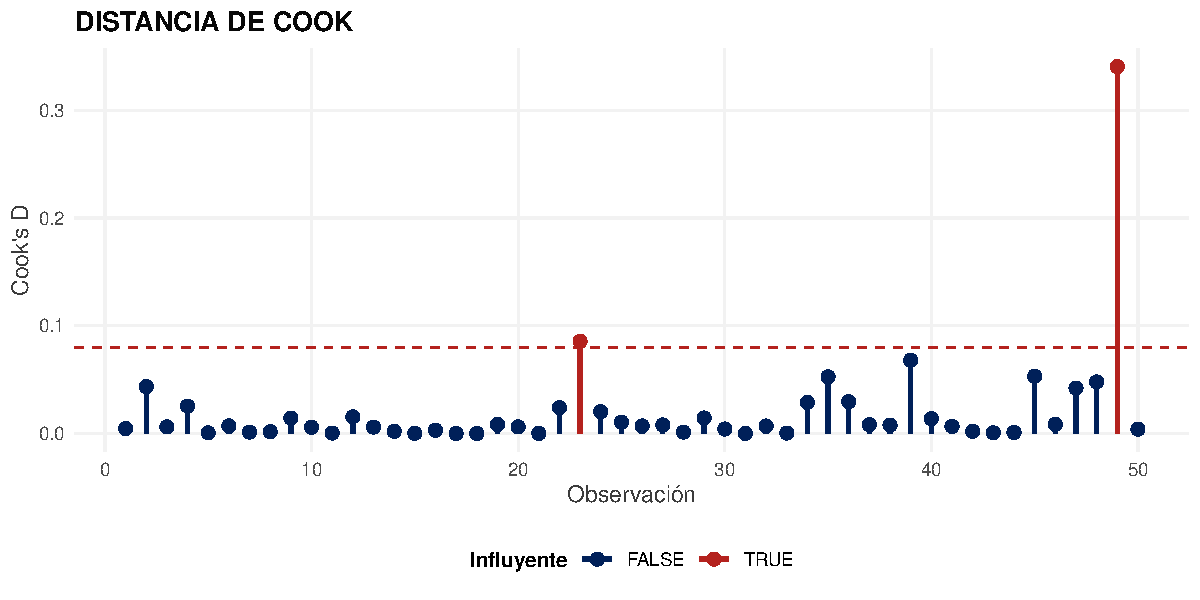
\includegraphics[width=\maxwidth]{figure/plot-cook-1} 

}

\caption[Distancia de Cook]{Distancia de Cook}\label{fig:plot-cook}
\end{figure}

\end{knitrout}

\section{Validación Cruzada}

\begin{knitrout}
\definecolor{shadecolor}{rgb}{0.969, 0.969, 0.969}\color{fgcolor}\begin{kframe}
\begin{alltt}
\hldef{n} \hlkwb{<-} \hlkwd{nrow}\hldef{(cars)}
\hldef{errores} \hlkwb{<-} \hlkwd{numeric}\hldef{(n)}

\hlkwa{for}\hldef{(i} \hlkwa{in} \hlnum{1}\hlopt{:}\hldef{n) \{}
  \hldef{m_temp} \hlkwb{<-} \hlkwd{lm}\hldef{(dist} \hlopt{~} \hldef{speed,} \hlkwc{data} \hldef{= cars[}\hlopt{-}\hldef{i,])}
  \hldef{errores[i]} \hlkwb{<-} \hldef{cars}\hlopt{$}\hldef{dist[i]} \hlopt{-} \hlkwd{predict}\hldef{(m_temp,} \hlkwc{newdata} \hldef{= cars[i,])}
\hldef{\}}

\hldef{rmse_cv} \hlkwb{<-} \hlkwd{sqrt}\hldef{(}\hlkwd{mean}\hldef{(errores}\hlopt{^}\hlnum{2}\hldef{))}
\hldef{mae_cv} \hlkwb{<-} \hlkwd{mean}\hldef{(}\hlkwd{abs}\hldef{(errores))}

\hlkwd{cat}\hldef{(}\hlsng{"=== VALIDACIÓN CRUZADA (LOOCV) ===\textbackslash{}n"}\hldef{)}
\end{alltt}
\begin{verbatim}
## === VALIDACIÓN CRUZADA (LOOCV) ===
\end{verbatim}
\begin{alltt}
\hlkwd{cat}\hldef{(}\hlsng{"RMSE:"}\hldef{,} \hlkwd{round}\hldef{(rmse_cv,} \hlnum{3}\hldef{),} \hlsng{"ft\textbackslash{}n"}\hldef{)}
\end{alltt}
\begin{verbatim}
## RMSE: 15.697 ft
\end{verbatim}
\begin{alltt}
\hlkwd{cat}\hldef{(}\hlsng{"MAE:"}\hldef{,} \hlkwd{round}\hldef{(mae_cv,} \hlnum{3}\hldef{),} \hlsng{"ft\textbackslash{}n"}\hldef{)}
\end{alltt}
\begin{verbatim}
## MAE: 12.059 ft
\end{verbatim}
\begin{alltt}
\hlkwd{cat}\hldef{(}\hlsng{"RMSE modelo completo:"}\hldef{,} \hlkwd{round}\hldef{(}\hlkwd{sigma}\hldef{(modelo),} \hlnum{3}\hldef{),} \hlsng{"ft\textbackslash{}n"}\hldef{)}
\end{alltt}
\begin{verbatim}
## RMSE modelo completo: 15.38 ft
\end{verbatim}
\end{kframe}
\end{knitrout}

\begin{knitrout}
\definecolor{shadecolor}{rgb}{0.969, 0.969, 0.969}\color{fgcolor}\begin{figure}[H]

{\centering 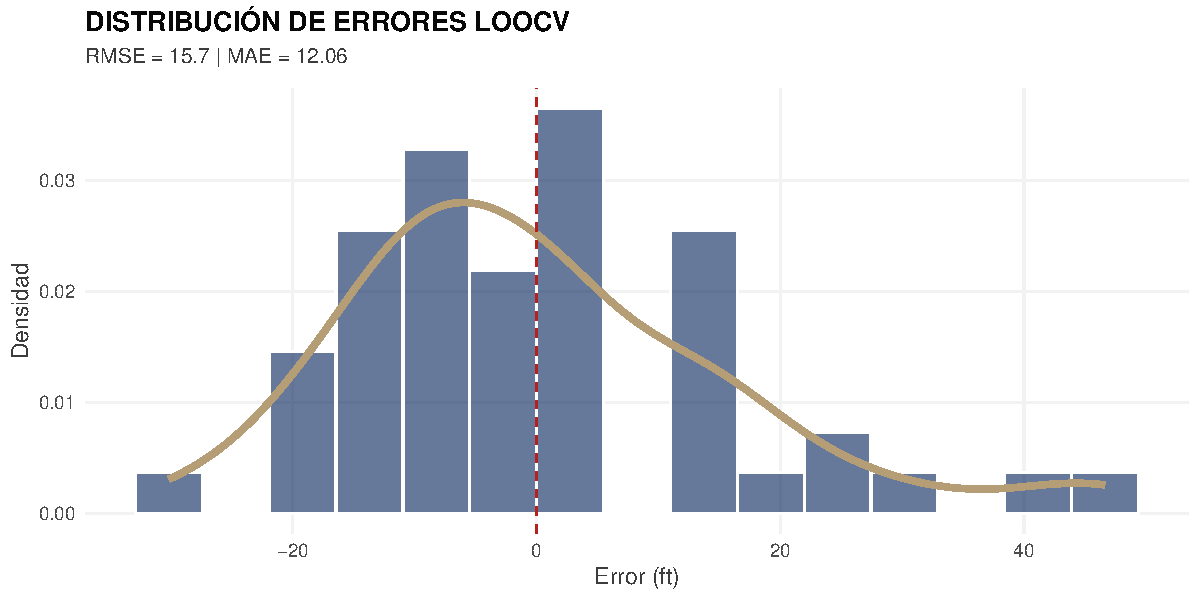
\includegraphics[width=\maxwidth]{figure/plot-cv-1} 

}

\caption[Errores de Validación Cruzada]{Errores de Validación Cruzada}\label{fig:plot-cv}
\end{figure}

\end{knitrout}

\section{Predicciones}

\begin{knitrout}
\definecolor{shadecolor}{rgb}{0.969, 0.969, 0.969}\color{fgcolor}\begin{kframe}
\begin{alltt}
\hldef{nuevos} \hlkwb{<-} \hlkwd{data.frame}\hldef{(}\hlkwc{speed} \hldef{=} \hlkwd{c}\hldef{(}\hlnum{10}\hldef{,} \hlnum{15}\hldef{,} \hlnum{20}\hldef{,} \hlnum{25}\hldef{,} \hlnum{30}\hldef{))}
\hldef{pred} \hlkwb{<-} \hlkwd{predict}\hldef{(modelo,} \hlkwc{newdata} \hldef{= nuevos,} \hlkwc{interval} \hldef{=} \hlsng{"prediction"}\hldef{)}

\hldef{resultados} \hlkwb{<-} \hlkwd{data.frame}\hldef{(}
  \hlkwc{Velocidad} \hldef{= nuevos}\hlopt{$}\hldef{speed,}
  \hlkwc{Predicción} \hldef{= pred[,}\hlnum{1}\hldef{],}
  \hlkwc{IC_Inf} \hldef{= pred[,}\hlnum{2}\hldef{],}
  \hlkwc{IC_Sup} \hldef{= pred[,}\hlnum{3}\hldef{]}
\hldef{)}

\hlkwd{print}\hldef{(resultados,} \hlkwc{digits} \hldef{=} \hlnum{1}\hldef{)}
\end{alltt}
\begin{verbatim}
##   Velocidad Predicción IC_Inf IC_Sup
## 1        10         22    -10     53
## 2        15         41     10     73
## 3        20         61     30     93
## 4        25         81     48    113
## 5        30        100     67    134
\end{verbatim}
\end{kframe}
\end{knitrout}

\begin{knitrout}
\definecolor{shadecolor}{rgb}{0.969, 0.969, 0.969}\color{fgcolor}\begin{figure}[H]

{\centering 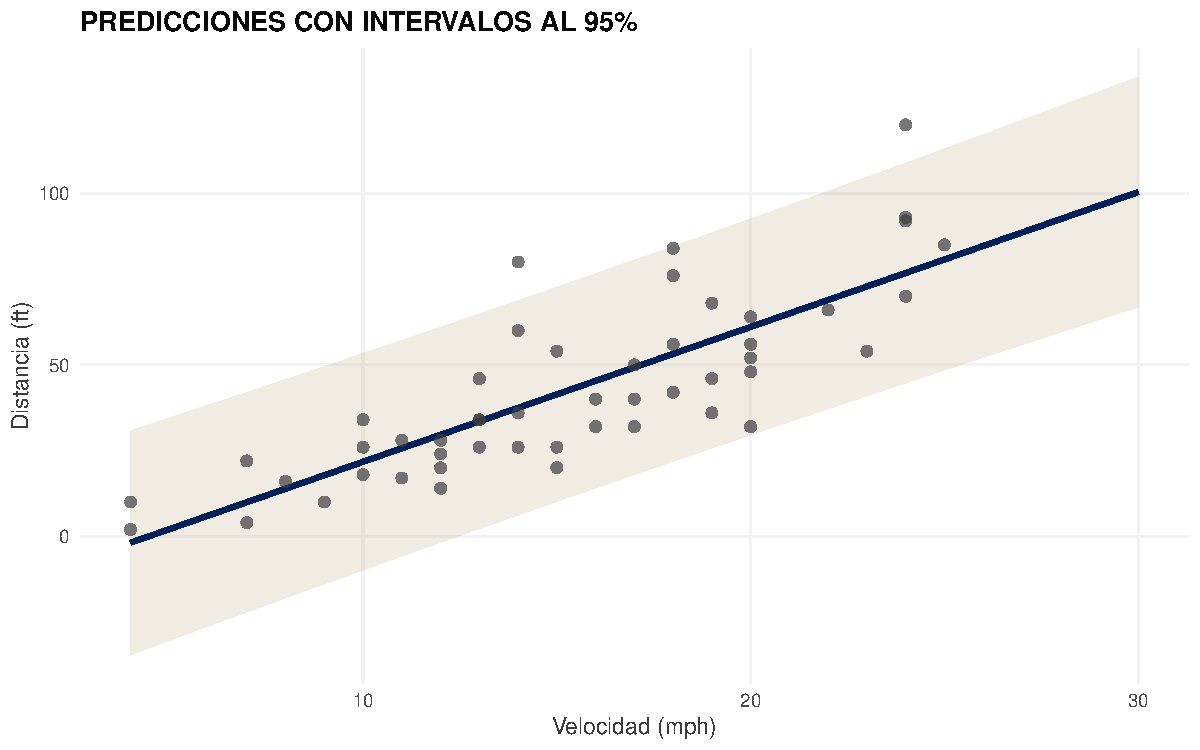
\includegraphics[width=\maxwidth]{figure/plot-pred-1} 

}

\caption[Predicciones con Intervalos]{Predicciones con Intervalos}\label{fig:plot-pred}
\end{figure}

\end{knitrout}

\section{Comparación de Modelos}

% latex table generated in R 4.5.1 by xtable 1.8-4 package
% Tue Jan  6 21:34:05 2026
\begin{table}[ht]
\centering
\caption{Comparación de Modelos} 
\begin{tabular}{lrrrr}
  \toprule
Modelo & R2 & AIC & BIC & RMSE \\ 
  \midrule
Lineal & 0.651 & 419.157 & 424.893 & 15.380 \\ 
  Cuadrático & 0.667 & 418.772 & 426.420 & 15.176 \\ 
   \bottomrule
\end{tabular}
\end{table}


\section{Conclusiones}

\begin{tcolorbox}[colback=SuccessGreen!10, colframe=SuccessGreen, arc=0pt,
                  boxrule=0.8pt, title=HALLAZGOS PRINCIPALES]
\begin{enumerate}[leftmargin=15pt, itemsep=3pt]
    \item Relación \critical{significativa} entre velocidad y distancia ($\beta_1 = 3.93$, p < 0.001)

    \item $R^2 = 0.6511$ (65.1\% de variabilidad explicada)

    \item Supuestos: Requieren atención

    \item Modelo cuadrático mejora $R^2$ en 1.63\%

    \item Validación cruzada: RMSE = 15.7 ft

    \item 2 observaciones influyentes detectadas
\end{enumerate}
\end{tcolorbox}

\subsection{Limitaciones y Recomendaciones}

\textbf{Limitaciones:}
\begin{itemize}[leftmargin=15pt, itemsep=2pt]
\item Dataset histórico (1920s) - tecnología obsoleta
\item Muestra pequeña (n=50)
\item Variables omitidas (clima, pavimento, peso)
\end{itemize}

\textbf{Recomendaciones:}
\begin{itemize}[leftmargin=15pt, itemsep=2pt]
\item Usar errores robustos para inferencia
\item Replicar con datos modernos (NHTSA)
\item Explorar modelos no lineales (GAMs, splines)
\item Validación con k-fold cross-validation
\end{itemize}

\section{Referencias}

\begin{itemize}[leftmargin=15pt, itemsep=2pt]
    \item Wooldridge, J.M. (2020). \textit{Introductory Econometrics}. 7th ed.
    \item Greene, W.H. (2018). \textit{Econometric Analysis}. 8th ed.
    \item R Core Team (2024). \textit{R: A Language for Statistical Computing}.
    \item Wickham, H. (2016). \textit{ggplot2: Elegant Graphics}. Springer.
\end{itemize}

\vfill
\hrule height 0.5pt
\vspace{6pt}
\begin{center}
\scriptsize\techfont
\textcolor{VogueBlack}{ECONOMETRÍA 2026} |
\textcolor{Champagne}{EMANUEL QUINTANA SILVA} |
UPTC

\vspace{2pt}
\textit{Documento generado con Sweave + R + LaTeX animate}
\end{center}

\end{document}
